% !TEX encoding = UTF-8 Unicode 

\section{Development approaches}

The definition of mobile development can be interpreted in a variety of ways. It can be seen as a broad process of implementing a mobile application, starting with planning and designing and finishing with testing, releasing and maintaining. A more software-oriented definition is that mobile development simply refers to implementing an application for mobile devices by coding it using a selected technology stack \cite{microsoft_mobile_development}. In this thesis, the latter definition is assumed.

Mobile development can become a complex task considering the variety of devices and platforms existing in the market. There are many different approaches available and in order to choose one over another the mobile application requirements should be taken into account as well as target platforms and devices, development and time costs \cite{velvetech_mobile_dev_approaches}.

In this chapter, there are presented selected popular approaches to mobile application development. Each of them is described mainly in the context of architecture, technology stack and tools, platforms supported and possible advantages or disadvantages.

\subsection{Native mobile development}

Native mobile development encompasses building mobile applications that can only be implemented using a platform-specific programming language and deployed to a single operating system \cite{comparative_analysis_native_hybrid}. Such an approach brings with it the necessity for creating and maintaining multiple codebases and with that possibly multiple development teams \cite{approach_to_assess_performance_case_study}. The number of distinct codebases does not simply equal to the number of target platforms, as different versions of a single platform may require to be implemented independently \cite{appdynamics_mobile_app_performance}. Hence, development costs are high from the viewpoint of financing and time.

Native mobile applications are closely integrated with the operating system through using target platform's components \cite{comparison_perf_looks_flutter_native}\cite{comp_analysis_hybrid_frameworks} and most recent features \cite{eval_rn_flutter}. For that reason, at times they can be referred to as "embedded" 
 \cite{cross_platform_development_study_rn_flutter} and in theory should provide the maximal performance. Furthermore, because native apps are developed according to the operating system's guidelines, such as Material design system for Android and Cupertino for iOS, they are naturally easy to use for users accustomed to that specific platform.

Since almost a decade, the mobile operating system market has been dominated by Android and iOS, reaching 99,3\% in March 2023 \cite{statcounter_mobile_os_market}. For this reason, in the context of this thesis only the above-mentioned operating systems are being taken into consideration.

As can be seen in the Figure \ref{fig:ios_versions}, in case of iOS, almost 90\% of devices are running either the most or second-most recent major version of the operating system. Therefore, when targeting the Apple's system, probably a single codebase would be enough.

However, in case of Android, there is a high level of market fragmentation, as nearly 20\% of smartphones or tablets are running older versions released as far as in 2015 (Figure \ref{fig:android_versions}). Because there are limitations such as deprecation of code commands and API (Application Programming Interfaces) behavior changes between distant versions, multiple codebases may be chosen to be maintained separately per a single mobile application. Another issue is the fact, that device manufacturers are able to apply various modifications to the operating system which can lead to errors occurring only on those devices \cite{comparison_technologies_multiplatform}, causing difficulties for developers. Because Apple is the exclusive manufacturer of devices running iOS, they do not suffer from such a problem. 

\begin{figure}[hb]
  \begin{minipage}{.47\textwidth}
    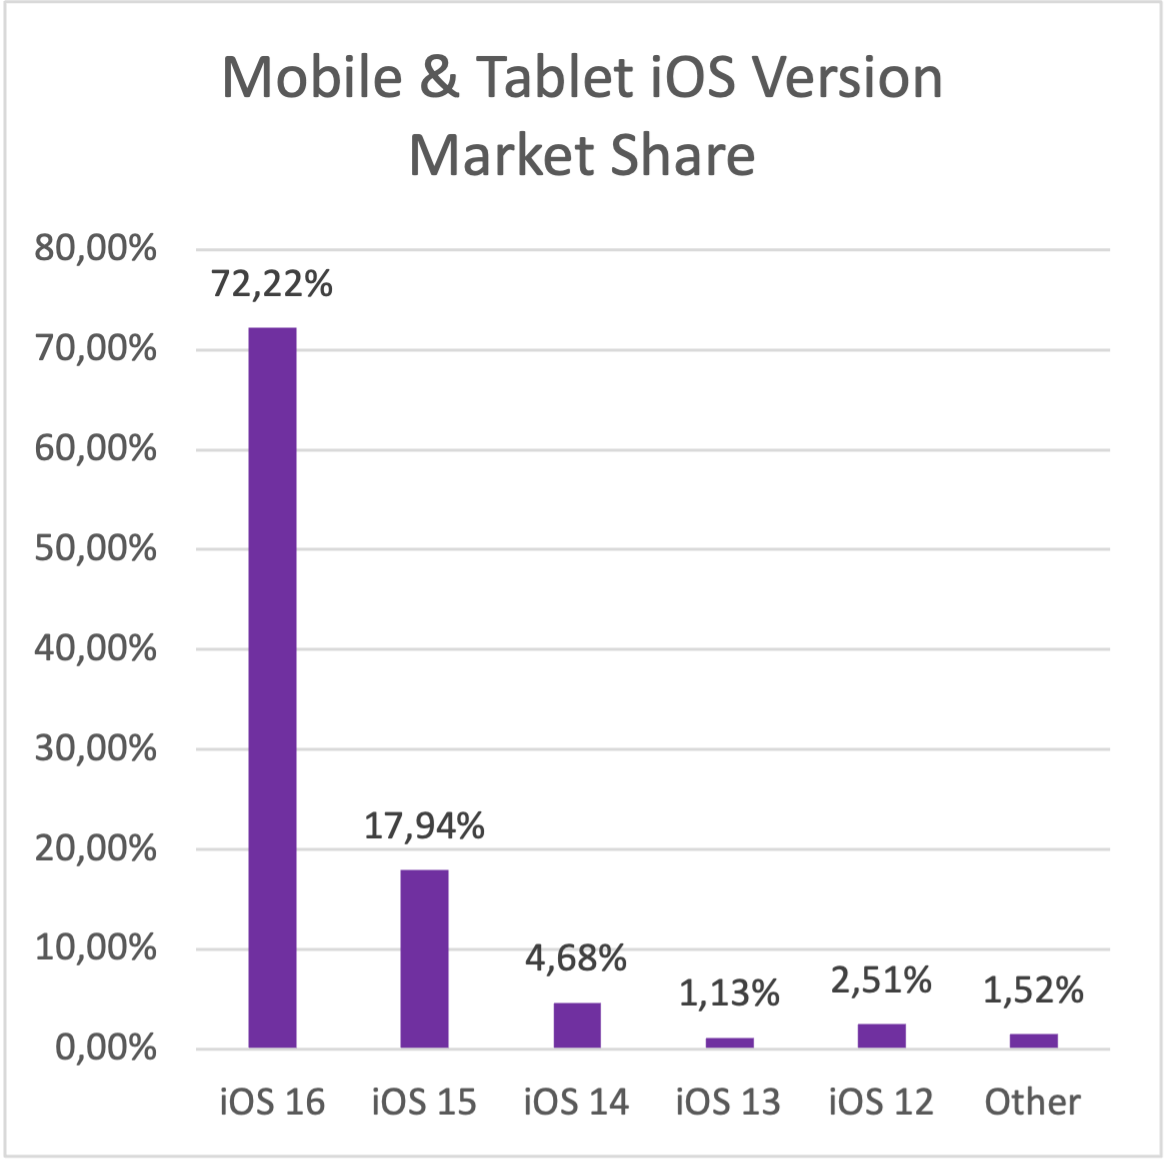
\includegraphics[width=\textwidth]{img/ios_ver_market_share}
    \caption{iOS version market share (Source: Own work based on \cite{statcounter_ios_version_market})}
    \label{fig:ios_versions}
  \end{minipage}
  \hfill
  \begin{minipage}{.47\textwidth}
    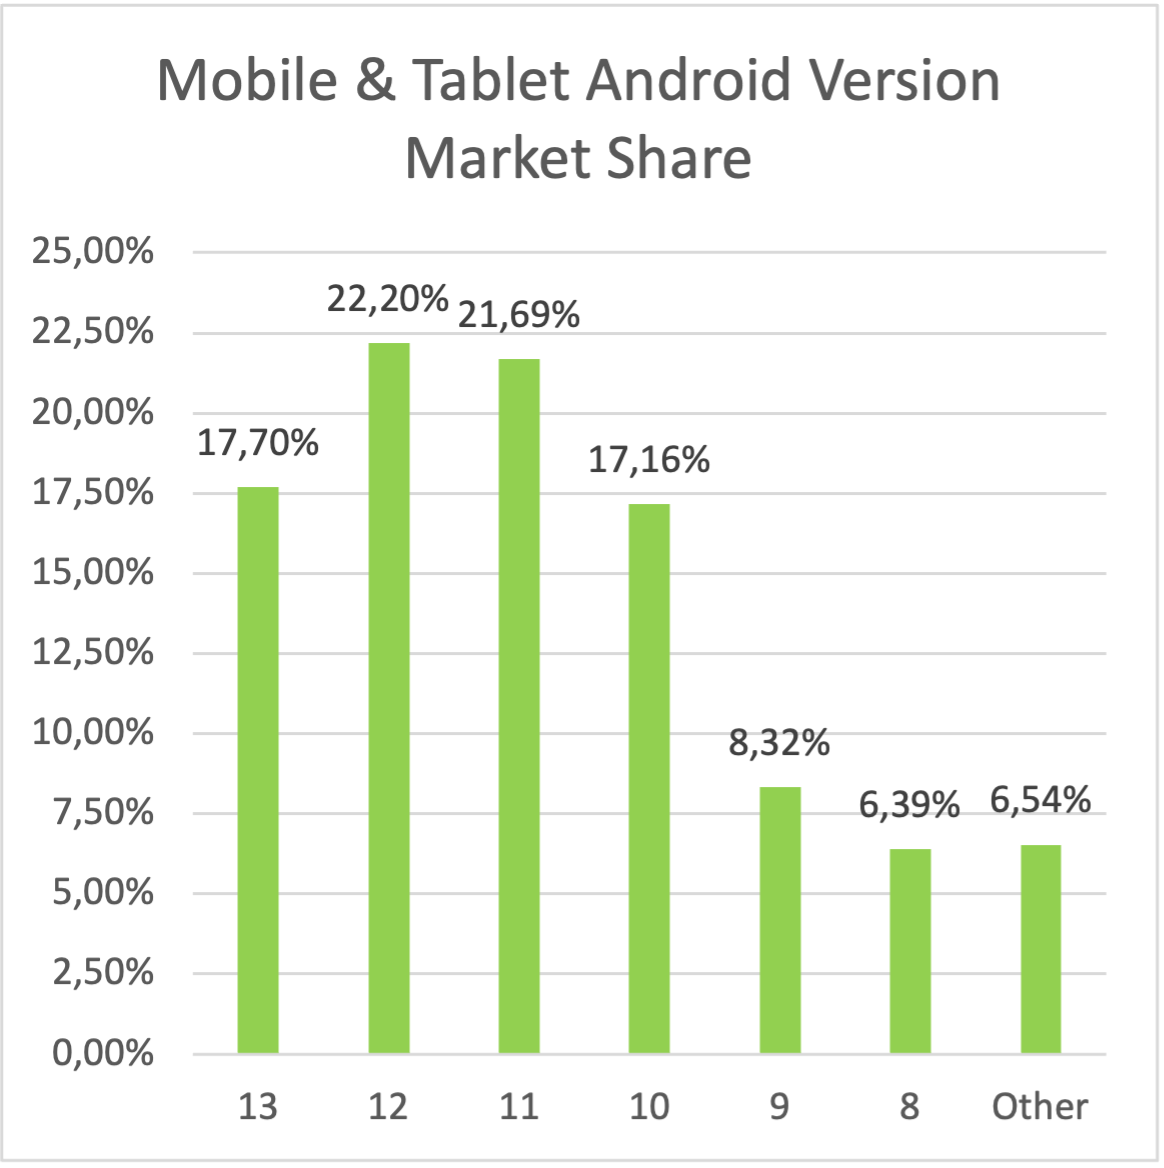
\includegraphics[width=\textwidth]{img/android_ver_market_share}
    \caption{Android version market share (Source: Own work based on \cite{statcounter_android_version_market})}
    \label{fig:android_versions}
  \end{minipage}
\end{figure}

\subsubsection{Android}

Android is an open-source operating system developed by the Open Handset Alliance and Google to run mainly on mobile devices such as smartphones and tablets but also TVs and cars \cite{android_what_is} \cite{comparison_technologies_multiplatform}. It is based on the Linux kernel and has a multiple-component structure \cite{android_architecture_and_application}, as can be seen in the Figure \ref{fig:android_architecture}. Each part takes responsibility for different tasks, e.g., Android Runtime provides optimized garbage collection and View System (included in Java API Framework) enables developers to implement the user interface layouts using various elements such as lists and buttons \cite{android_architecture}.

\begin{figure}
    \centering
    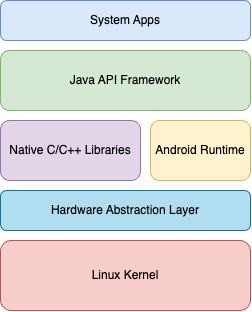
\includegraphics[scale=0.6]{img/android_architecture}
    \caption{Android architecture (Source: Own work based on \cite{android_architecture})}
    \label{fig:android_architecture}
\end{figure}

It is not necessary to use an IDEs (Integrated Development Environment) to build most software. Despite that, most programmers tend to reach out to them because of the guaranteed development comfort and productivity increase. Android Studio is the primary IDE for native mobile development of Android applications. It is created on top of IntelliJ's IDEA and provides numerous features such as Gradle, advanced debugging tools and profilers, etc \cite{android_studio_intro}.

For many years, Java has been the official language for Android development. However, since Google established Kotlin as the default choice in 2019 \cite{android_kotlin_first}, over 60\% of programmers have switched to it \cite{android_kotlin}. Furthermore, data shows that almost 90\% of the Google Play Store Top 500 USA mobile apps have been developed with it \cite{kc_kotlin_vs_java}. Kotlin's popularity is certainly going to grow in the upcoming years, considering the undeniable benefits it brings. Still, there are some scenarios in which Java could remain the first choice.

Table \ref{tab:java_kotlin_comparison} shows that all the features necessary for Android application development, such as e.g., Android SDK or AndroidX support, are fully provided by both Java and Kotlin. Furthermore, the latter introduces additional advantages in the form of enabling the usage of Jetpack Compose toolkit and even the ability to create multi-platform projects (Kotlin Multiplatform is currently only accessible in Beta version \cite{kotlin_multiplatform}).

Java is a high-level object-oriented programming language introduced as far back as 1995. It is one of the most popular languages in the world which is regularly updated, reaching version 20 this year. However, in the context of Android development the supported versions are 8 and 11, with the latter requiring high Android API version in order to use all the offered elements (although upgraded API desugaring announced in February this year broadens the range of libraries available without increasing the app's minimum supported API level \cite{android_api_desugaring}). The advantages of Java mainly result from the fact it is present for a very long time. During the last 30 years it gathered a big community of developers with high-level experience. Therefore, it may be easier to form a competent team for the project. Moreover, there are numerous applications that had been created with Java which owners might not seek for a migration, which as a result maintains Java's importance in the market \cite{kc_kotlin_vs_java}.

On the other hand, Kotlin offers many assets because of which it has replaced Java as an official first-choice language for Android development, as mentioned before. Kotlin is a comparatively recent programming language introduced in 2016 by JetBrains. First and foremost, it is fully interoperable with Java and therefore, it is possible to call Kotlin code inside Java code and vice versa. Secondly, Kotlin's syntax is very concise and null-safe, thus increasing the speed of development and reducing the project's code lines and lowering the possibility of mistakes. For those reasons, implementation of new apps using Kotlin is fairly straight-forward and comfortable from the point of view of developers. Moreover, the migration of existing projects from Java to Kotlin is uncomplicated and can lead to size decrease and simplification of the codebase with much smaller Null Pointer Exception occurrence in runtime \cite{android_kotlin_first}.

\begin{table}[hb]
  \centering
    \caption{Java and Kotlin comparison (Source: Own work based on \cite{android_kotlin_first})}
    \label{tab:java_kotlin_comparison}
    \begin{tabular}{ | p{55mm} | >{\centering}p{33mm} | >{\centering\arraybackslash}p{33mm} | }
      \hline
      \multicolumn{1}{ |c| }{\textbf{Feature}}&\textbf{Java}&\textbf{Kotlin}\\
      \hline
      Platform SDK support&Yes&Yes\\
      \hline
      Android Studio support&Yes&Yes\\
      \hline
      Lint&Yes&Yes\\
      \hline
      Guided docs support&Yes&Yes\\
      \hline
      API docs support&Yes&Yes\\
      \hline
      AndroidX support&Yes&Yes\\
      \hline
      AndroidX Kotlin-specific APIs (KTX, croutines, \dots)&N/A&Yes\\
      \hline
      Online training&Best effort&Yes\\
      \hline
      Samples&Best effort&Yes\\
      \hline
      Multi-platform projects&No&Yes\\
      \hline
      Jetpack Compose&No&Yes\\
      \hline
      Compiler plugin support&No&Yes (Kotlin Symbol Processing API)\\
      \hline
    \end{tabular}
\end{table}

Since Kotlin has already been established as the preferred programming language for Android development, all considerations in the scope of this thesis will be limited to it rather than Java.

% TODO: XML vs Jetpack Compose

% TODO: Material design

\subsubsection{iOS}
Include Cupertino!!!
